To calculate price changes for our consumption goods, we use an input-output model, CO2-emissions on sector level and CO2-coefficients for consumer goods. 

%We have 8 consumption goods:
%\begin{itemize}
%    \item Meat and dairy
%    \item Other foods
%    \item Housing
%    \item Energy for housing
%    \item Energy for transport
%    \item Transport
%    \item Other goods
%    \item Other services
%\end{itemize}


\subsection{Emissions data}
Statistics Denmark provide data for greenhouse gas emissions in CO2-equivalents for 117 industries as well as private households in the table DRIVHUS. We obtain these data for the latest year, 2018. These emissions exclude emissions from the burning of biomass, but include emission froms Danish operated vessels and planes abroad, which are not part of the UNFCCC emission reporting standards and do not count towards the 70 pct reduction target, which makes it unlikely that a carbon tax will be imposed on those emissions. Using the bridge table MRO2 we subtract emissions not part of the UNFCCC emission reporting standard from the relevant industries.
\begin{table}[]
    \centering
    \caption{Danish greenhouse gas emissions, 2018}
    \begin{tabular}{lccc}
    
\textit{1,000 tons CO2e}    	        &DRIVHUS	& UNFCCC &	UNFCCC incl. LULUCF \\ \hline
Total	        &89,578	    & 47,863	     &54,456\\ \hline
Households	&8,161	    & 8,161	     &8,161\\
Industries total	&81,417	    & 39,702	     &46,295 \\ \hline
    \end{tabular}
    \label{emissions2018}
\captionsetup{singlelinecheck=off,size=scriptsize}
\setlength{\captionmargin}{10pt}
\caption*{
\textbf{Note:} Emissions are excluding burning of biomass. Emissions from international transport are subtracted from the relevant industries. All LULUCF emissions are ascribed to the industry 'Agriculture and horticulture'. \\ \textbf{Source:} Statistics Denmark, tables DRIVHUS and MRO2 and own calculations}
\end{table}
Emissions from Danish territory can be attributed to consumption of these consumption composites through two channels: 1) Direct emissions from household consumption of fossil fuels and 2) Indirect emissions stemming from domestic production of intermediate and final goods that are consumed domestically. These are described in the following sections.


\subsection{Direct household emissions}
Using data from Statistics Denmark, table ENE2HA, we allot the household emissions from to the relevant consumption groups. First, using relevant carbon intensities for different energy goods\footnote{Kindly provided by Sune Caspersen from Arbejderbevægelsens Erhvervsråd}, we can determine how total household emissions are made up of consumption of specific fossil fuels. We find that approximately 75 pct. of household emissions come from consumption of gasoline and diesel, and the remaining 25 pct. comes from consumption of other oil products and natural gas. We ascribe these emission to our to consumption composites energy for transport and energy for housing, see Table \ref{tabdirectemissions}.

\begin{table}[H]
\centering
\caption{Taxation of direct household emissions}
\begin{tabular}{ll}
\textit{1,000 tons CO2}  & Emissions \\ \hline
Total             & 8,161 \\ \hline
Gasoline and diesel   & 6,075  \\ 
Natural gas, other gases and other oil products & 2,086   \\ \hline
\end{tabular}
\label{tabdirectemissions}
\setlength{\captionmargin}{10pt}
\caption*{
\textbf{Note:} Emissions from transport fuels are ascribed to transport, the rest is ascribed to heating and electricity. \\ \textbf{Source:} Statistics Denmark, tables DRIVHUS, MRO2, ENE2HA and own calculations}
\end{table}
To implement a carbon tax on these emissions, we simply multiply emissions with a tax rate,
\begin{align}
    Tax^{Direct}_g = \tau E^{Direct}_g,
\end{align}
where $Tax^{Direct}_c$ are total tax payments for each consumer good $c \in [1,74]$, $\tau$ is the tax rate and $E^{Direct}_c,$ are emissions from each consumer good. The consumer goods are at the 74-good-level from the national accounts.

\subsection{Taxation of indirect emissions}\label{secindirecttax}
To calculate the emissions stemming from Danish production of Danish services, we set up an input-output model inspired by \cite{Wier2005}. The total indirect emissions are calculated by 
\begin{align} 
\label{leontiefindirect}
    Tax^{Indirect} = \tau \Gamma (I-A)^{-1} C,
\end{align}
where $\tau$ is the carbon tax rate, a scalar. $\Gamma$ is $(1 \times 117)$ vector of carbon intensities calculated as industry-specific emissions divided by total production (both intermediate and final goods) in that industry.
$(I-A)^{-1}$ is the symmetric Leontief matrix, which measures the input-output intensity between each of the 117 sectors of the economy. I is the identity matrix and A is the $(117 \times 117)$ matrix of technical coefficients, calculated from the  input-output data table NI01, Statistics Denmark. Each entry in A is calculated by
\begin{align}
    a_{ij} = \frac{z_{ij}}{x_{j}}, 
\end{align}
where $z_{ij}$ is total input from sector $i$ to $j$, and $x_j$ is total production of sector $j$ \citep{miller_blair_2009}.

$C$ is a  $(117 \times 74)$  matrix mapping domestic production to domestic consumption. Each entry in $c_{ig}$ is the final good deliveries from each industry $i$ to each consumer good $g$. Consequently, total indirect emissions from domestic production which can be attributed to domestic consumption are given by
\begin{align}
    E^{Indirect} = \Gamma (I-A)^{-1} C.
\end{align}
Then, the resulting $1 \times 74$ vector from equation (\ref{leontiefindirect})
\begin{align}
   Tax^{indirect} = \tau E^{Indirect} 
\end{align}
is the indirect tax payments for each commodity group. 


\subsection{Emission projections from Danish Energy Agency}\label{sec:kf21fremskriv}
The \cite{kf21} forecasts Danish Greenhouse Gas emissions until 2030 assuming a frozen policy scenario in their report Danish Climate Outlook 2021 (Klimastatus- og fremskrivning 2021, or KF21). They do so for 8 aggregated sectors: Households, transport, services, manufacturing and construction, oil production and refineries, electricity and district heating, waste management, and agriculture, horticulture and fisheries. All sectors, except agriculture, are projected to reduce their emissions towards 2030. Most notably, emissions from electricity production and district heating are expected to decrease by 95 pct. from 2019 to 2030. As emissions in certain sectors are projected to fall significantly, using only 2018 emissions data would seriously overestimate the impact of carbon taxation in even the near future.

We map the projected emission reductions from these aggregated sectors to the 117 industries as well as the household emissions. For most industries, the mapping is relatively straight forward. Emissions from the national account industries agriculture and horticulture are assumed to follow the projections for agriculture and horticulture in KF21. The same logic applies to production of oil, transport, manufacturing, waste management and services. For household emissions, we assume that emissions from transport fall as the KF21 transport sector, and that emissions from heating (natural gas and other oil products) fall as the KF21 household sector. Emissions from transport fuels are projected to fall partly due to increased use of biofuels and partly due to the expected transition to electric vehicles. Emissions from the household sector in KF21 are almost entirely made up of individual heating. They are projected to fall due to transitions to heat pumps and district heating.

\begin{figure}[H]
\centering
\caption{CO2e emissions from selected industries and consumption goods}
\label{emissions2030}
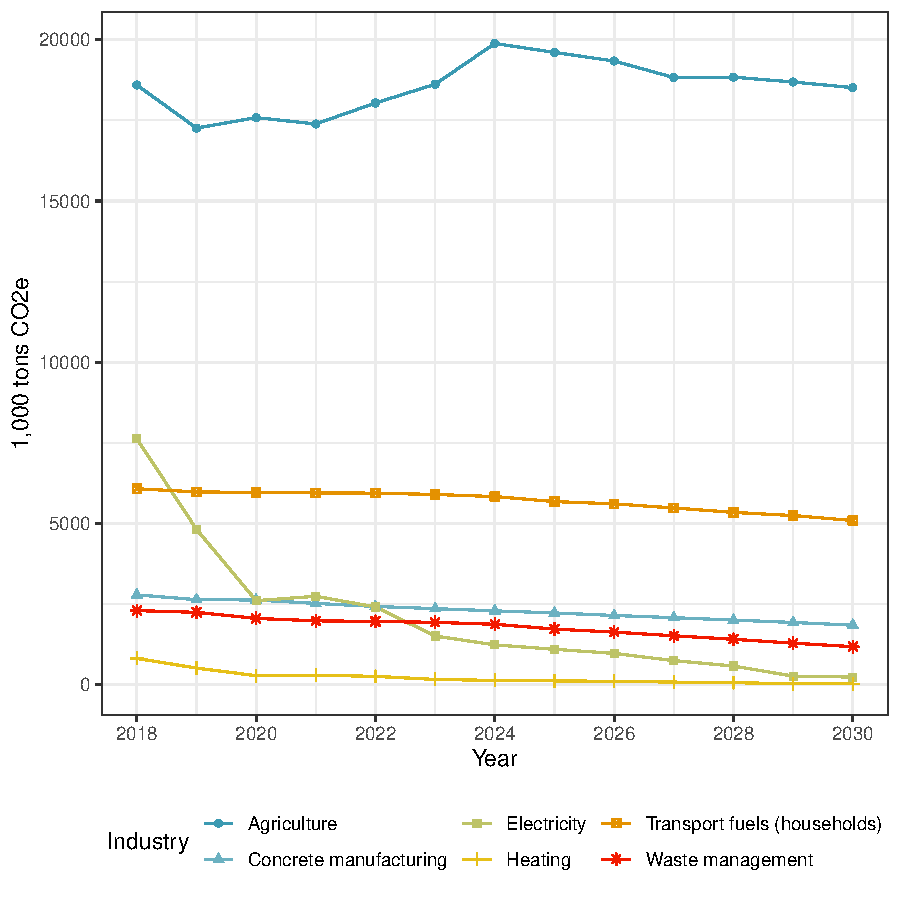
\includegraphics[width=.9\textwidth]{Figures/emissionkf21.pdf}
\captionsetup{singlelinecheck=off,size=scriptsize}
\setlength{\captionmargin}{10pt}
\caption*{
\textbf{Note:} ??\\
\textbf{Source:} Statistics Denmark, \cite{kf21} and own calculations}
\end{figure}
The projected emissions from selected high-carbon industries and household emissions from energy for transport are presented in Figure \ref{emissions2030}. Agriculture is projected to be the most carbon intensive industry in 2030, essentially maintaining the level until 2030. Electricity and heating industries will both have significantly reduced their emissions already by 2020 and are close to zero in 2030. Concrete manufacturing and waste management are also projected to reduce emissions, but not as much as the electricity sector. Emissions from household's consumption of gasoline and diesel fall around 15 pct. 

We can then recalculate expected tax payments for each year towards 2030. For the direct tax payments, they are given by
\begin{align}
    Tax^{Direct}_{gt} = \tau_t E^{Direct}_{gt},
\end{align}
where $E^{Direct}_{gt}$ are the projected emissions for each consumption good. For the indirect tax payments, they are given by
\begin{align} 
    Tax^{Indirect}_t = \tau_t \Gamma_t (I-A)^{-1} C,
\end{align}
where $\Gamma_t$ are the industry-specific carbon intensities, which follow the projection from KF21. We can also use the model to calculate carbon intensities for each good, which arise from setting the carbon tax rate $\tau=1$. In figure \ref{carbonintens2030} the carbon intensities for the 4 most carbon intensive good composites in our 8-grouping are shown. Energy for transport, which are essentially just transport fuels, are by far the most carbon intensive. Energy for housing, which consists primarily of electricity, district heating and natural gas consumption, is pretty carbon intensive in 2018, but falls to a level of 0.017 tons per 1000 DKK consumed in 2030, close to the level of "Other foods". 

\begin{figure}[H]
\centering
\caption{CO2e emission intensities for good composites}
\label{carbonintens2030}
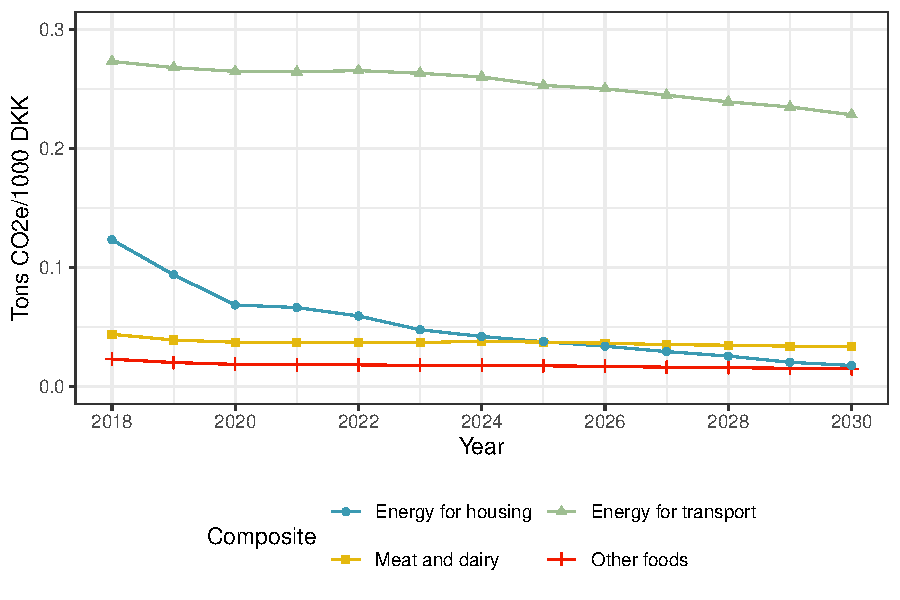
\includegraphics[width=.9\textwidth]{Figures/intens21.pdf}
\captionsetup{singlelinecheck=off,size=scriptsize}
\setlength{\captionmargin}{10pt}
\caption*{
\textbf{Note:} Carbon intensities are calculated as the sum of direct and indirect emissions, divided by total consumption of a given group. \\
\textbf{Source:} Statistics Denmark, \cite{kf21} and own calculations}
\end{figure}

\subsection{Calculating price changes}
For each commodity group we can calculate the total tax payments as
\begin{align}
    Tax^{tot}_{gt} = Tax^{indirect}_{gt} + Tax_{gt}^{direct},
\end{align}
where $Tax_{gt}^{direct}$ is zero for all goods except transport fuels, gas and other heating-related oil products.

We proceed to assume that the tax burden falls entirely on consumers, such that we can calculate price changes for each good with
\begin{align}
    p_{gt} = 1 + \frac{Tax^{tot}_{gt}}{X_g},
\end{align}
where $X_g$ is total domestic consumption of each commodity group from the national accounts. This gives us projected price changes for the 74 consumption goods in the national accounts. To apply our estimation of the linear expenditure system with 8 goods, we aggregate these price changes using a Laspeyres price index. Prices of each our 8 consumption good composites, denoted by subscript $gc$ are given by
\begin{align}\label{eq:pricechanges}
    p_{gc,t} = \frac{\sum_{g=1}^{G_{gc}} p_{gt} X_{g}}{\sum_{g=1}^{G_{gc}} X_g } = \sum_{g=1}^{G_{gc}} p_{gt} w_g , 
\end{align}
where the indices $g=1$ to $G_{gc}$ indicate those goods from the 74-grouping that make up a given good composite $gc$. More simply put, this is just a weighted average of the prices of the 74-grouping, where weights are calculated as the consumption of the 74-grouping good $g$ divided by the sum of the consumption goods that are in a given good composite $gc$ in the base year.

Table \ref{pchange1250} presents price changes for a carbon tax reform where a 1250 DKK tax is imposed on all emissions. The tax is linearly phased in from 2026-2030. The good composite with the largest price increase is energy for transport, which increases with 28.5 pct in our input-output model. Meat and dairy increases by 4.2 pct. and energy for housing just 2.2 pct. Energy for housing increases by such a small amount due to the rapid projected decarbonization in the electricity and district heating sectors. The carbon intensity of transport fuels, already very high, is not projected to fall much towards 2030, which is why the price increase is quite significant. 

\begin{table}[H]
    \centering
    \caption{Price changes from a uniform carbon tax increase 1250 DKK phased in from 2026}
    \label{pchange1250}
    \begin{tabular}{lcccccc} \hline
 Good & 2025  &2026   &2027   &2028  & 2029 &  2030\\ \hline

  Meat and dairy & 1 &1.0091 &1.0176 &1.0261 &1.0339 &1.0416\\
   Other foods & 1 &1.0042 &1.0081 &1.0119 &1.0154 &1.0187\\
  Housing & 1 &1.0018 &1.0035 &1.0051 &1.0064 &1.0077\\
   Energy for housing & 1 &1.0085 &1.0147 &1.0192 &1.0204 &1.0222\\
   Energy for transport & 1 &1.0625 &1.1224 &1.1793 &1.2348 &1.2853\\
   Cars and Transport services & 1 &1.0017 &1.0032 &1.0046 &1.0058 &1.0070\\
  Other goods& 1 &1.0023 &1.0043 &1.0062 &1.0078 &1.0093\\
  Other services & 1 &1.0019 &1.0036 &1.0052 &1.0064 &1.0077 \\ \hline
    \end{tabular}
    \captionsetup{singlelinecheck=off,size=scriptsize}
\setlength{\captionmargin}{10pt}
\caption*{
\textbf{Note:} Price changes are calculated following equation \ref{eq:pricechanges}.}
\end{table}
Of course, our relatively aggregated consumption categories have certain implications. For example, the fall in the carbon intensity of energy for housing is not driven by a decreasing carbon intensity of oil and natural gas, but rather intra-category substitution towards district heating and heat pumps \citep{kf21}. Similarly, the emission reductions in energy for transport are not only due to higher expected biofuel content in the transport fuels, but also substitution towards electric vehicles, which are less carbon-intensive. These substitutions may in themselves imply higher prices for consumers, which we ignore in our analysis. 


\subsection{Assumptions}\label{sec:io-assumptions}
An important fundamental assumption of the input-output model is that all the technical coefficients in the $A$ matrix is constant \citep{miller_blair_2009}. This means that the production function is Leontief-type - there is no substitution between inputs, even if one input becomes more inexpensive than the other. 
\\
\\
Another implicit assumption of our approach is that levies imposed on the industry is fully transmitted to consumer prices, as in \cite{Wier2005}. We thus ignore the general equilibrium effect that substituion away from carbon-intensive goods would limit the price increase of those exact goods. 
Actual consumer prices are of course not only a function of domestic producer prices and taxes, but also of foreign producer prices. Our input-output model cannot capture this effect, as it is based on Danish production only. We assume that the tax levies are passed on to consumers in full, and that the consumers do not substitute towards imported goods instead. This is obviously not a very realistic assumption - if Danish production becomes increasingly expensive, standard economics of trade would predict a substitution towards foreign goods. However, our results should not be interpreted as if Danish consumers will carry all of the tax burden of increased carbon taxation of Danish industries. In our model, we only include the production that is actually consumed by Danish consumers as final demand, ignoring production for exports, investment and public spending. That means only emissions that are associated with Danish consumption is actually taxed, and emissions associated with exports are not. This means that the price increases predicted by the model are smaller than a consumption tax, where all emissions, foreign and domestic, are taxed at the level of final consumption. Here, we only account for domestic emissions.
\\
\\
At the same time, it has been suggested that for certain goods that a have a high risk of carbon leakage, such as agricultural goods, a carbon tax on production should be complemented with a carbon tax on consumption to reduce that leakage \citep{klimaraad2021}. Furthermore, it does not seem socially acceptable that e.g. the agricultural sector will be subject to very high carbon taxation, while consumers just substitute towards foreignly produced agricultural products. Thus it seems realistic that agricultural products will have increased consumer prices under increased carbon taxation, even if foreign competitors do not experience similiar increases in carbon taxation. 
\\
\\
Overall, the assumptions associated with this input-output-analysis indicate that the impact of carbon taxation is likely an upper bound estimate of what the actual impact of increased (national) carbon taxation on consumers would be: Consumers are assumed to carry all of the tax burden, there is no substitution towards less carbon-intensive and cheaper inputs in production, and there is no substitituion towards cheaper, less sharply regulated foreign goods. 



\subsection{Results}
A very simple green tax reform could involve raising the carbon tax from the current level of 180 DKK to 1500 DKK, as \cite{klimaraad2021} has suggested. To operationalize this in our input-output model, we impose a flat tax of 1250 DKK, such that the sum of the current carbon tax and the imposed tax is close to 1500 DKK. The tax is gradually imposed starting in 2026 with 20 pct. and fully implemented in 2030. The price changes are presented in table \ref{pchange1250}. We assume that prices are constant from 2030-2040.

The resulting impact across the income distribution is graphed in the following, measured as the equivalent variation relative to total expenditure and disposable income, respectively. As the tax is phased from 2026-2030, the impact rises from that point. 

Measured as share of expenditure, it can be seen that the carbon tax hits fairly evenly across the income distribution. When fully phased in, the EV is approximately 1.8 pct. of expenditure for all income quintiles. When measured as a share of disposable income, the impact is more regressive. For the richest quintile, the EV is 1 pct. of disposable income, and  1.9 pct for the poorest quintile. These results reflect that the richest quintiles consume a relatively smaller share of their income while the poorest actually spend more than their disposable income. From 2030 and onwards, the equivalent variation is sligtly falling (numerically) as the minimum consumption level of more expensive goods, such as energy for transport falls. 

\begin{figure}[H]
\centering
\caption{EV of a uniform 1250 DKK carbon tax reform phased in}
\label{figshare_1250}
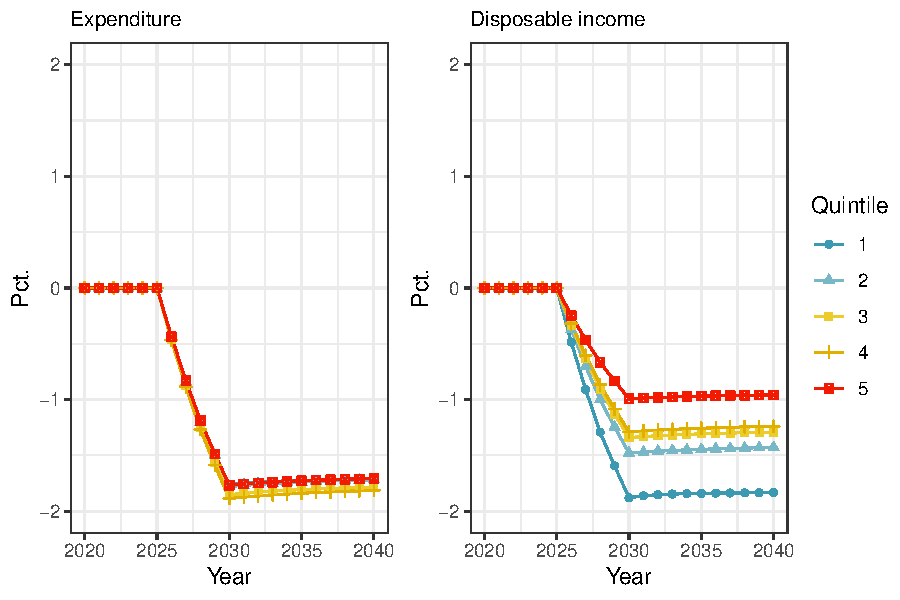
\includegraphics[width=.7\textwidth]{Figures/IO-resultater/timeEV_1250_indfas.pdf}
\captionsetup{singlelinecheck=off,size=scriptsize}
\setlength{\captionmargin}{10pt}
\caption*{
\textbf{Note:} ??\\}
\end{figure}

\begin{figure}[H]
\centering
\caption{EV of a uniform 1250 DKK carbon tax in 2030}
\label{figshare_bar_1250}
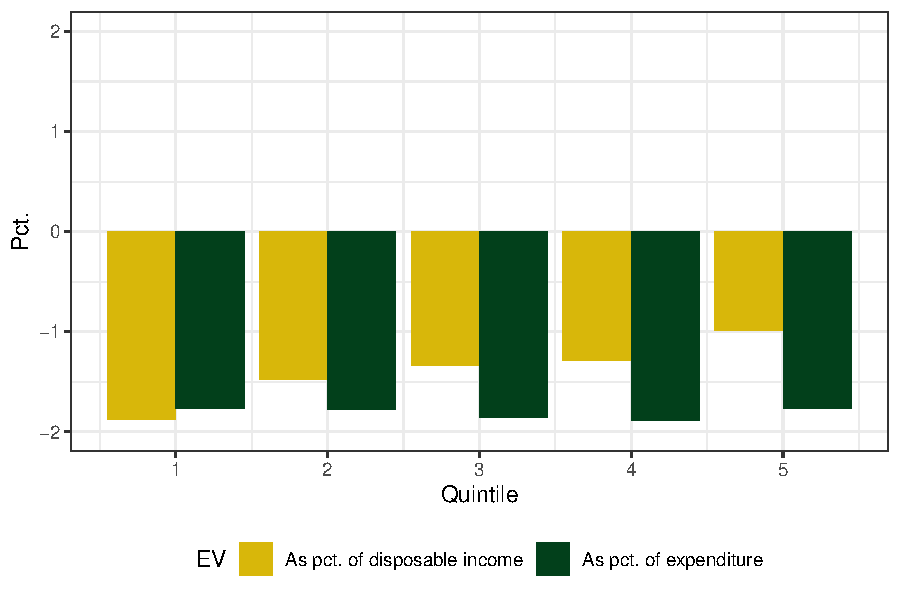
\includegraphics[width=.7\textwidth]{Figures/IO-resultater/bar2030_1250_indfas.pdf}
\captionsetup{singlelinecheck=off,size=scriptsize}
\setlength{\captionmargin}{10pt}
\caption*{
\textbf{Note:} ??\\}
\end{figure}
The relative equal impact across the income distribution of the carbon tax can be explained by the fact that the lower quintiles spend a relatively larger share of total expenditure and meat and dairy, other foods and energy for housing, which all become more expensive under the tax reform. At the same time, energy for transport becomes even more expensive, which the richer quntiles spend a larger fraction of their expenditure on. These effects offset, such that the reform is roughly distributionally neutral. This is illustrated in figure \ref{fig:cs_decomp}, where the consumer surplus (see section \ref{sec:measurewelfare}) is decomposed onto each of the 8 consumption composites. 

\begin{figure}[H]
\centering
\caption{Consumer surplus decomposed, 2030}
\label{fig:cs_decomp}
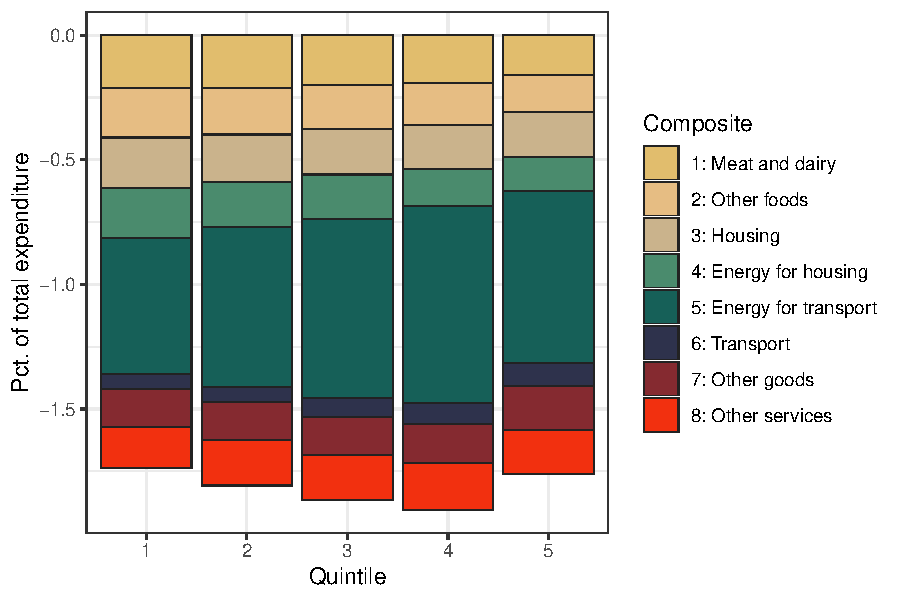
\includegraphics[width=.8\textwidth]{Figures/IO-resultater/cs_decomposed_exp.pdf}
\captionsetup{singlelinecheck=off,size=scriptsize}
\setlength{\captionmargin}{10pt}
\caption*{
\textbf{Note:} ??\\}
\end{figure}

\subsubsection{1250 DKK carbon tax immediately imposed from 2022}
If we immediately impose a carbon tax from 2022, the price changes are larger compared to the 2026-2030 phase-in. This is mostly due to the fact that  the electricity and district heating sectors are projected to rapidly decarbonize, such that their emissions in 2030 is only approximately 3 pct. of what they were in 2018. This also means that the impact of consumers will be higher compared to a tax reform that is gradually phased in from 2026.

The EV of a more immediate carbon tax reform is (numerically) larger than the phased-in version. In terms of the EV to expenditure-ratio, it still is approximately neutral across the income distribution. In terms of EV to disposable income, the tax is most regressive when it is imposed in 2022, but the regressivity falls as the impact does towards 2030.

\begin{figure}[H]
\centering
\caption{EV of a uniform 1250 DKK carbon tax reform from 2022}
\label{figtax2022}
\includegraphics[width=.7\textwidth]{Figures/IO-resultater/timeEV_1250_straks.pdf}
\captionsetup{singlelinecheck=off,size=scriptsize}
\setlength{\captionmargin}{10pt}
\caption*{
\textbf{Note:} ??}
\end{figure}

\subsubsection{Regressive tax reforms}\label{sec:regressivetaxref}
Given the concerns of carbon tax reforms being regressive, we find it relevant to explore which types of reform that would actually yield regressive outcomes, measured as the EV to expenditure ratio. The most carbon intensive goods composites are energy for transport, meat and dairy and energy for housing in that order. The poorest income quintiles spend a larger share of their total expenditure on the two latter groups, while the reverse is true for energy for transport. Thus, a regressive carbon tax reform will require that those goods increase relatively more in price than energy for transport.

If we tax only the greenhouse gas emissions from the agricultural sector, it will mostly affect prices of food. In the following example, we impose a 1250 DKK tax rate on only the agricultural sector from 2022 and onwards. At a glance, this may seem like a highly unrealistic tax reform. However, it should be noted that total taxes levied on e.g. electricity and fuels exceed the proposed level of 1500 DKK/ton CO2e for most uses, especially true for households \citep{dmoer2021} . In the agricultural sector, only a very small share of the sectors emissions are currently taxed \citep{klimaraad2021}. Thus, a truly uniform carbon tax with a level of 1500 DKK/ton would involve lower taxes on gasoline, e.g., and a much lower tax on electricity. Considering that, food prices might be most affected by a uniform carbon tax reform, depending on the exact design.



\begin{figure}[H]
\centering
\caption{EV of a 1250 DKK tax on agricultural emissions}
\label{figagriculturetax}
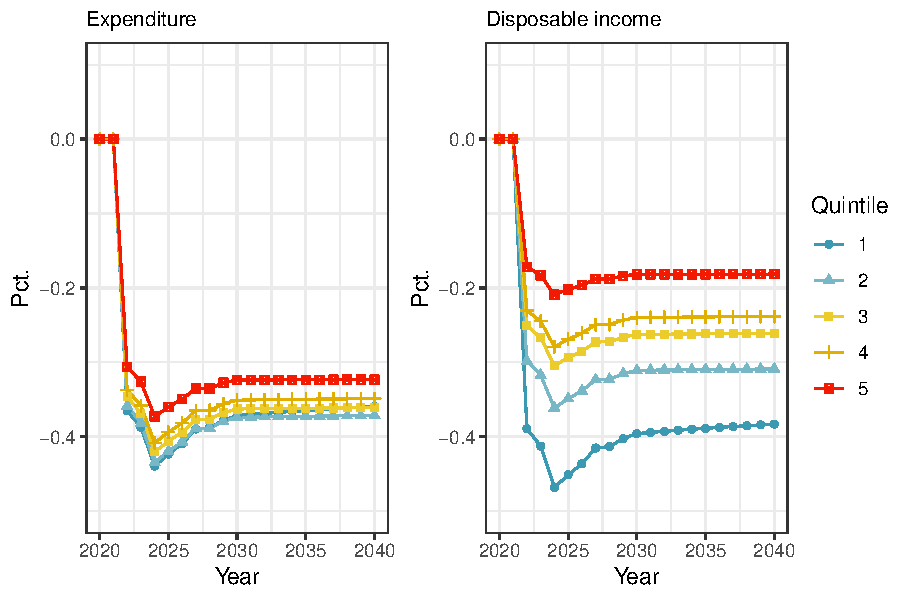
\includegraphics[width=.7\textwidth]{Figures/IO-resultater/landbrugev.pdf}
\captionsetup{singlelinecheck=off,size=scriptsize}
\setlength{\captionmargin}{10pt}
\caption*{
\textbf{Note:} ??\\}
\end{figure}

From figure \ref{figagriculturetax}, it is obvious that the impact measures as EV to total expenditure is, unsurprisingly, much smaller than in the previous tax reforms, due to only agricultural emissions being taxed as opposed to all emissions. We do also see that, as opposed to earlier, this tax reform is slightly regressive measured in terms of EV to expenditure. However, the difference in impact is less than .1 pct. In terms of EV to disposable income, the regressivity is amplified, as previously. 

\subsubsection{Carbon tax exempting transport fuels}
Considering that gasoline and diesel are already subject to very high tax rates in Denmark, a relevant scenario might be a carbon tax reform where transport fuels are exempt from tax increases. Experience from other countries, e.g. France's yellow vest-movement, suggest that public support of increased gasoline and diesel taxation can be limited. Further, a uniform carbon tax, where all fossil fuels are taxed according to their carbon emissions, would most likely involve lower taxation of fossil fuels for transport, given a proposed level of 1500 DKK/ton.

\begin{figure}[H]
\centering
\caption{EV of a 1250 DKK carbon tax, transport fuels exempted}
\label{figtaxwobenz}
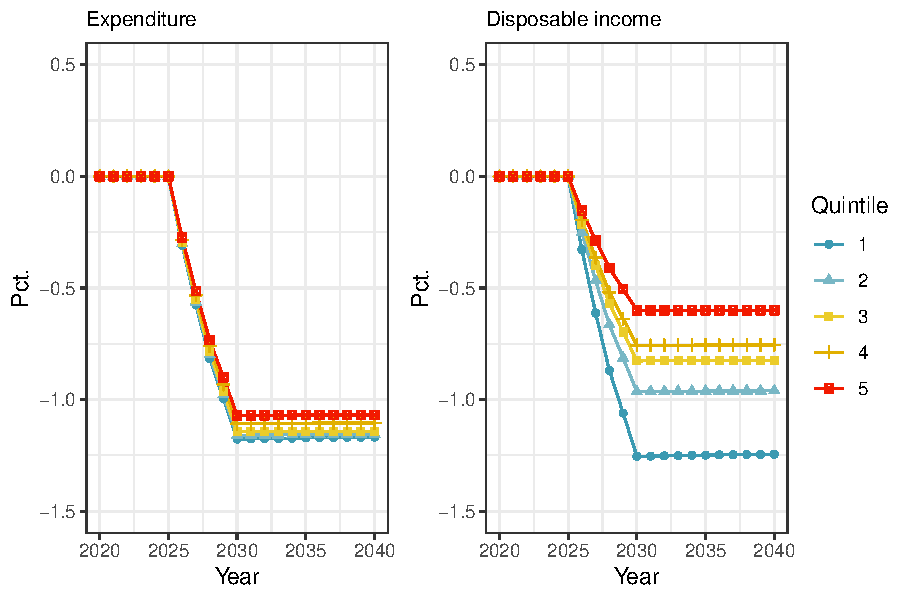
\includegraphics[width=.7\textwidth]{Figures/IO-resultater/benz_undtag_evtime.pdf}
\captionsetup{singlelinecheck=off,size=scriptsize}
\setlength{\captionmargin}{10pt}
\caption*{
\textbf{Note:} ??\\}
\end{figure}

As figure \ref{figtaxwobenz} shows, this tax reform will be slightly regressive in terms of EV to to expenditure. This is due to meat and dairy, other foods and energy for housing rising in price, while the price of energy for transport is unaffected.

Our results suggest that carbon tax increases will only be regressive if they have a significant impact on food prices relative to prices on transport fuel. As the richer quintiles spend a larger share of their expenditure on transport fuels, increased taxation of those fuels will yield more progressive outcomes. Rising food prices and prices for energy for housing will have the opposite effect. Our results suggest that if all domestic carbon emissions caused by domestic consumption is increased, the impact will be roughly evenly distributed across the income distribution - even before redistribution of the revenue.

\subsubsection{Comparison with Kraka (2020)}\label{sec:krakacompare}
To assess whether it our method yields different results regarding the regressivity of a carbon tax reform than the method applied in \cite{Kraka2020}, we calculate the consumer surplus in two ways. First, we calculate it with household-specific changes in quantities due to the price changes. These quantity changes arise from using our demand system estimations in a partial model, just as we do when calculating the EV. The consumer surplus is then calculated by applying the 'rule-of-half', as described in section \ref{sec:measurewelfare}. Then, applying the method of \cite{Kraka2020}, we calculate average quantity changes, and assume that the relative change in quantities are the same across the income distribution.

To compare results, we look at 1) the uniform carbon taxation phased in from 2026-2030 and 2) the tax reform where transport fuels are exempted.

From figure \ref{krakasamlign1} we see the that the differences in welfare are relatively small. For each welfare metric, the conclusion that the carbon tax is approximately neutral across the income distribution does not change. All welfare changes are also within .2 pct., measured relative to total expenditure. If we zoom in, we see that Kraka's method estimate the welfare change to be .1 pct. lower than the other two welfare metrics - but is higher for other quintiles.

\begin{figure}[H]
\centering
\caption{Welfare comparison, 1250 DKK carbon tax phased in}
\label{krakasamlign1}
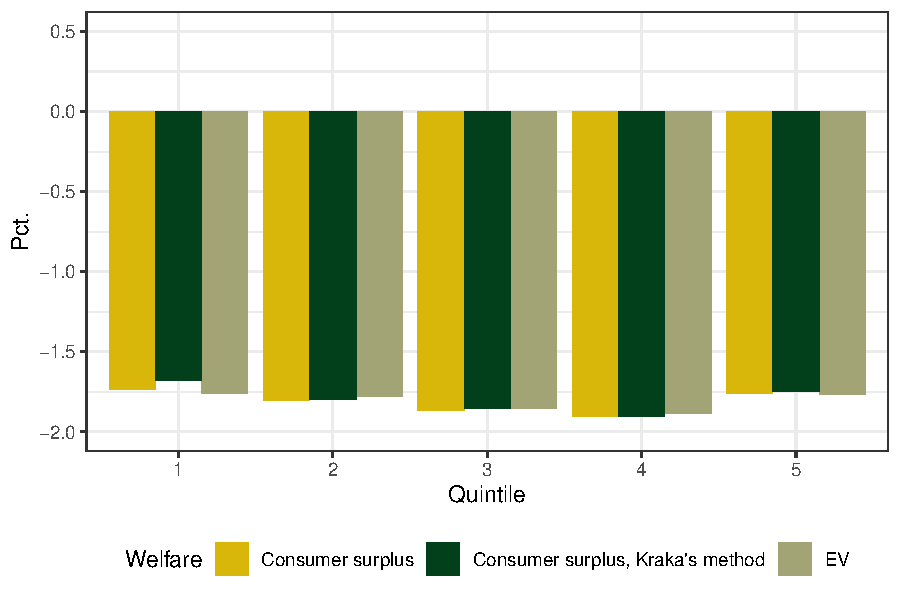
\includegraphics[width=.7\textwidth]{Figures/IO-resultater/bar_sammenlign_indfas.pdf}
\captionsetup{singlelinecheck=off,size=scriptsize}
\setlength{\captionmargin}{10pt}
\caption*{
\textbf{Note:} All welfare metrics are measured relative to total expenditure. The welfare change is measured in 2030.\\}
\end{figure}

The same picture arises when we assess the impact of the same tax reform, but with transport fuels exempt. Here, however, Kraka's method yields a smaller impact across the income distribution - however, only about .03 pct. lower. 

\begin{figure}[H]
\centering
\caption{Welfare comparison, with transport fuels exempt}
\label{krakasamlign2}
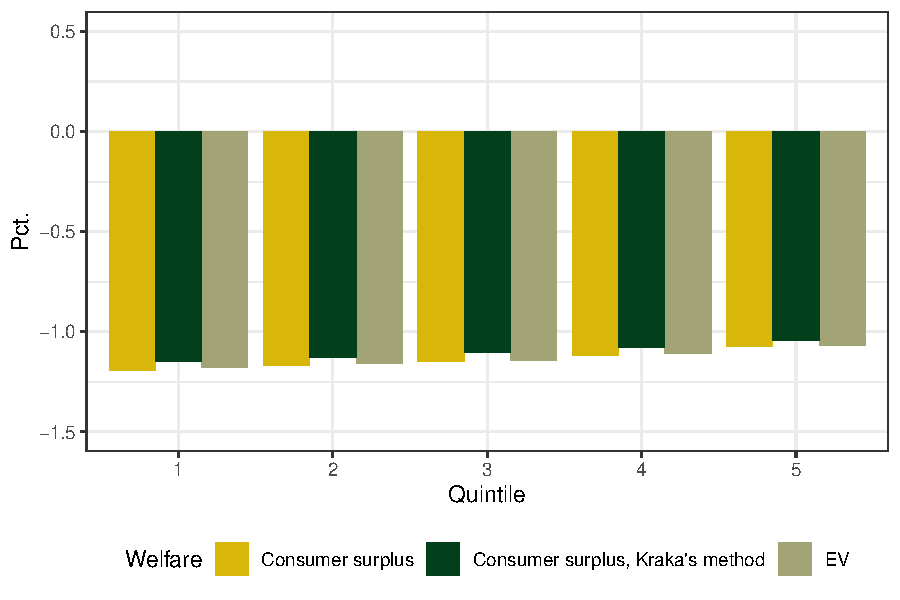
\includegraphics[width=.7\textwidth]{Figures/IO-resultater/bar_sammenlign_benzundtag.pdf}
\captionsetup{singlelinecheck=off,size=scriptsize}
\setlength{\captionmargin}{10pt}
\caption*{
\textbf{Note:} All welfare metrics are measured relative to total expenditure. The welfare change is measured in 2030.\\}
\end{figure}
The results indicate that estimating demand systems for different income quintiles - at least with our method - does not yield different welfare changes compared to estimating for a represenative household, and applying relative changes to observed consumption levels of different households. As our estimates of price and income elasticities in our LES demand system do not vary significantly across the income distribution, it would be surprising if the impact of increased carbon taxation was very dependent on whether quantity changes are calculated at the household level or at the macro level. Furthermore, \cite{araar2019prices} show that the calculation EV and consumer surplus yields approximately the same results, as long as price changes are relatively small.


\subsubsection{Comparison with other demand systems}
In this section, we compare our Linear Expenditure System with the Cobb Douglas demand as well as Leontief demand. 

For the Cobb-Douglas demand, the demand function is just the LES with $b=0$
\begin{align}
   x_{it} = \frac{\alpha^{CD}_i \mu_t}{p_{it}},
\end{align}
where $\alpha^{CD}_i$ calibrated to the consumption shares of each good for each household in 2019.

For Leontief demand, the Marshallian demand
function is 
\begin{align}
    x_{it} = \alpha^{L}_i(\sum x_{i,t}),
\end{align}
where $\alpha^{L}_i$ is calibrated the same way as $\alpha^{CD}_i$. Both demand functions are subject to the budget constraint
\begin{align}
    \sum p_{it} x_{it} = \mu_t.
\end{align}
We implement these demand function in the partial model described in section \ref{sec:partialmodel}. We then proceed to calculate the consumer surplus by the 'rule-of-half' for each of the utility functions described in section \ref{sec:measurewelfare} to ensure that the welfare metrics are comparable. The results are seen in figure \ref{samlignnytte}.

\begin{figure}[H]
\centering
\caption{Comparison of utility functions}
\label{samlignnytte}
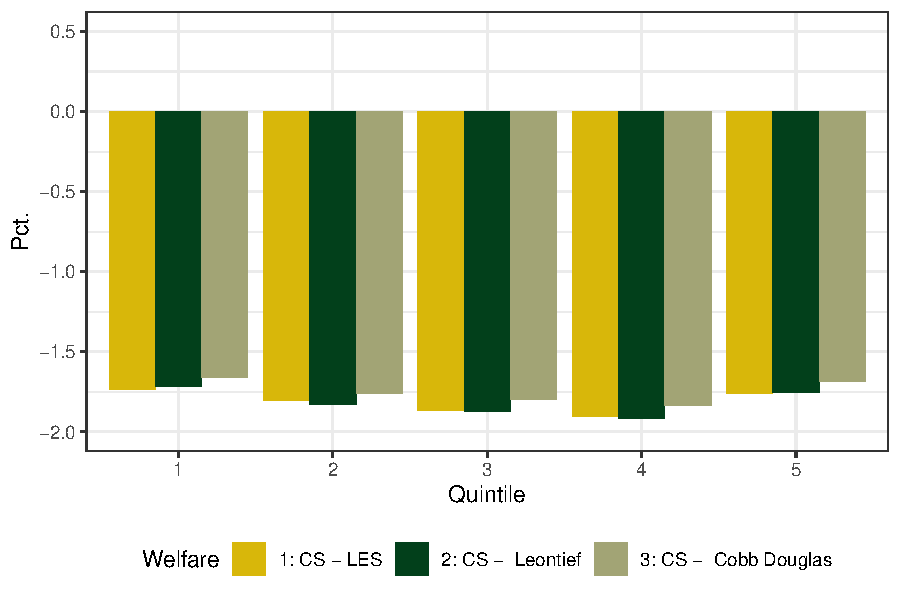
\includegraphics[width=.7\textwidth]{Figures/IO-resultater/bar_samlign_nyttefunk.pdf}
\captionsetup{singlelinecheck=off,size=scriptsize}
\setlength{\captionmargin}{10pt}
\caption*{
\textbf{Note:} Consumer surplus is measured relative to total expenditure. The welfare change is measured in 2030. The reform is a 1250 DKK carbon tax phased in from 2026 to 2030. \\}
\end{figure}
The estimated impact of a tax reform on consumer surplus is almost identical between the LES and Leontief demand. The impact is a tiny bit larger with Leontief demand for the middle quintiles, but a bit smaller for the bottom quintiles. This result is not very surprising giving the fact that we estimated quite high $b's$, and as a consequence, most of the demand is 'necessary'. 

The impact on consumer surplus is smaller when assuming Cobb-Douglas preferences. Cobb Douglas preferences imply unitary own-price, thus much higher than those estimated with the LES. This implies more substituion away from the more expensive goods because of the carbon tax reform. Thus, as consumers reduce their consumption of the carbon-intensive goods more relative to the LES or Leontief demands, the impact measured as consumer surplus will be smaller. This is evident in figure \ref{samlignnytte}. However, as can also be seen, the distribution of the impact is approximately the same regardless of the chosen utility function. 

Thus, using the LES and our estimates of it to evaluate rising prices will give a higher \textit{level} of the impact compared to Cobb-Douglas preferences, however, the \textit{distribution} of the impact is virtually unchanged. 


\subsubsection{Tax refoms with income growth}
We impose a tax reform with a 1250 DKK/ton CO2e in both income growth scenarios.  

To evaluate the impact of a carbon tax reform, we calculate the EV for a baseline scenario with constant prices and for the tax reform scenario with increased prices (from 2026 and onwards). As before, we divide the EV with respect to expenditure and disposable income, respectively. However, as we let income and expenditure grow, we divide the EV calculated in a given year with the income measure in the same year. The results are presented in the following figures in tables. 

The two income growth scenarios are barely distinguishable in terms of the calculated EV. The \textit{size} of the impact of the carbon tax reform is smaller compared to the scenario with no income growth, which is quite mechanically a consequence of the denominator growing. This, however, illustrates an important point: As income and consumption grows towards 2030, consumers will be better off, and the effects of increased taxation will be smaller as a share of income - and thus might 'hurt' less. 

\begin{figure}[H]
\centering
\caption{Uniform income growth}
\label{fig:uniincgr}
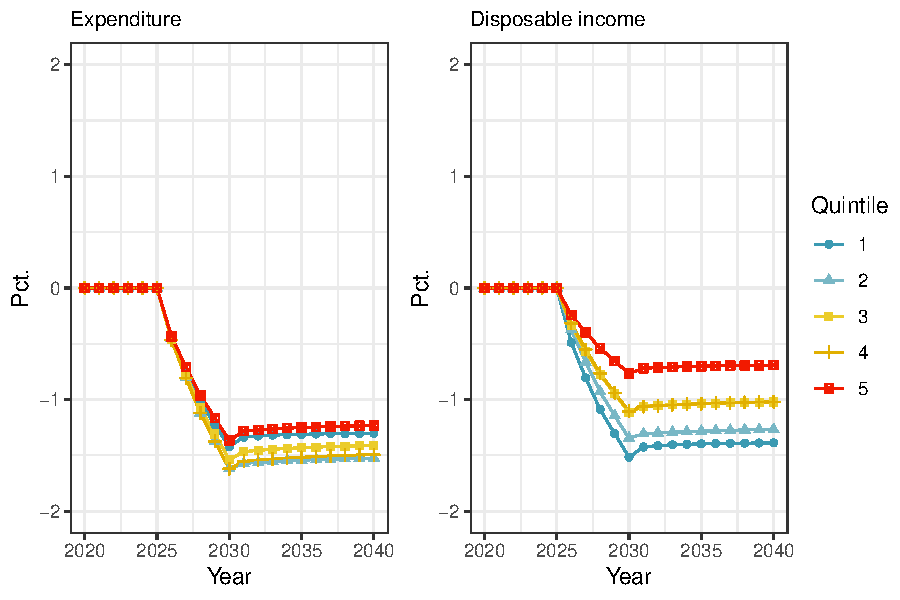
\includegraphics[width=.7\textwidth]{Figures/timeEV_1250_indfas_unifincgrowth.pdf}
\captionsetup{singlelinecheck=off,size=scriptsize}
\setlength{\captionmargin}{10pt}
\caption*{
\textbf{Note:} ??\\}
\end{figure}

The \textit{distribution} of the impact does not change much. Compared to total expenditure, the impact is still quite equal across the income distribution. However, the impact on the middle quintilesis a bit higher than in the scenario with no income growth. For quintile 2, it is mostly due to a more consistently high share of meat and dairy, while it for quintile 3 and 4 is due to a relatively high consumption share of energy for transport. The impact measured as a share of disposable income is still quite regressive, even as the size of the impact shrinks.

\begin{figure}[H]
\centering
\caption{Differentiated income growth}
\label{fig:diffincgro}
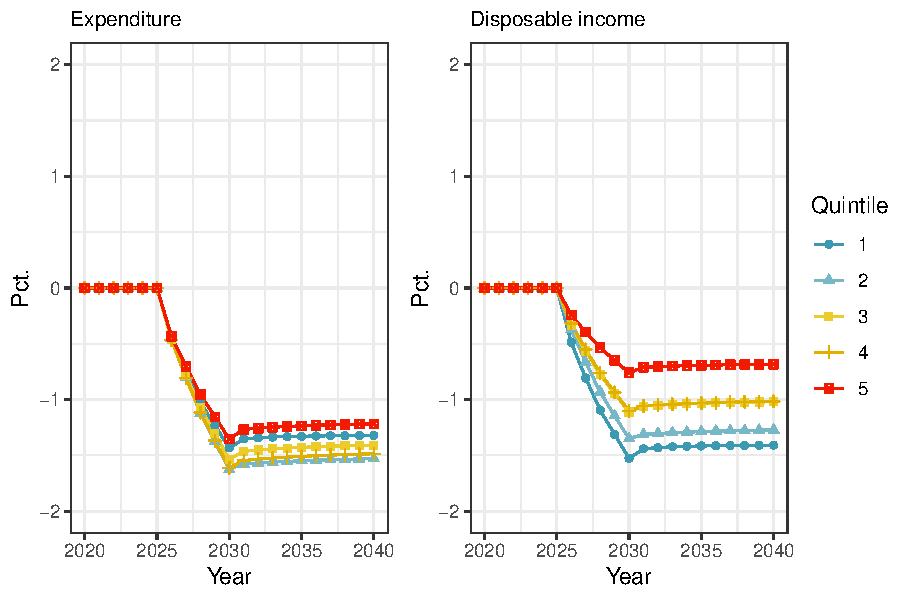
\includegraphics[width=.7\textwidth]{Figures/timeEV_1250_indfas_diffincgrowth.pdf}
\captionsetup{singlelinecheck=off,size=scriptsize}
\setlength{\captionmargin}{10pt}
\caption*{
\textbf{Note:} ??\\}
\end{figure}

This can also be seen from table \ref{incgrowth_storfed}. The two good composites that rise mostly in price due to the carbon tax reform is meat and dairy (3.5 pct.) and energy for transport (28 pct.). In all three income growth scenarios, the fairly neutral distribution across income groups are explained by a relatively high consumption share of meat and dairy in the poorest quintiles, but a relatively low consumptions share of energy for transport. 

\begin{table}[H]
    \centering
    \caption{Income growth}
    \label{incgrowth_storfed}
    \resizebox{\textwidth}{!}{%
    \begin{tabular}{l|l|llll|llll|llll}
\toprule \hline
                                                                                          & Quintile          & \multicolumn{4}{c|}{1}            & \multicolumn{4}{c|}{3}            & \multicolumn{4}{c}{5}            \\ \hline
                                                                                          & Year              & 2018  & 2026   & 2030   & 2040   & 2018  & 2026   & 2030   & 2040   & 2018  & 2026   & 2030   & 2040   \\ \hline
\multirow{6}{*}{\begin{tabular}[c]{@{}l@{}}No\\ income \\ growth\end{tabular}}            & Meat and dairy    & 0.054 & 0.051  & 0.050  & 0.047  & 0.048 & 0.049  & 0.050  & 0.049  & 0.039 & 0.040  & 0.040  & 0.040  \\
                                                                                          & Energy transport  & 0.018 & 0.025  & 0.026  & 0.024  & 0.026 & 0.028  & 0.032  & 0.029  & 0.024 & 0.028  & 0.031  & 0.028  \\
                                                                                          & Total Expenditure & 209   & 209    & 209    & 209    & 336   & 336    & 336    & 336    & 476   & 476    & 476    & 476    \\
                                                                                          & Disp. Income      & 196   & 196    & 196    & 196    & 464   & 464    & 464    & 464    & 849   & 849    & 849    & 849    \\
                                                                                          & EV/exp            & 0.000 & -0.455 & -1.764 & -1.721 & 0.000 & -0.463 & -1.852 & -1.785 & 0.000 & -0.437 & -1.768 & -1.708 \\
                                                                                          & EV/dispinc        & 0.000 & -0.485 & -1.880 & -1.834 & 0.000 & -0.335 & -1.340 & -1.292 & 0.000 & -0.245 & -0.992 & -0.958 \\ \hline
\multirow{6}{*}{\begin{tabular}[c]{@{}l@{}}Uniform\\ income\\ growth\end{tabular}}        & Meat and dairy    & 0.054 & 0.047  & 0.045  & 0.040  & 0.048 & 0.048  & 0.049  & 0.048  & 0.039 & 0.040  & 0.040  & 0.040  \\
                                                                                          & Energy transport  & 0.018 & 0.027  & 0.028  & 0.027  & 0.026 & 0.029  & 0.032  & 0.029  & 0.024 & 0.027  & 0.030  & 0.028  \\
                                                                                          & Total Expenditure & 209   & 234    & 248    & 286    & 336   & 376    & 399    & 460    & 476   & 534    & 565    & 652    \\
                                                                                          & Disp. Income      & 196   & 220    & 233    & 268    & 464   & 520    & 551    & 635    & 849   & 952    & 1008   & 1163   \\
                                                                                          & EV/exp            & 0.000 & -0.459 & -1.423 & -1.302 & 0.000 & -0.462 & -1.538 & -1.412 & 0.000 & -0.434 & -1.368 & -1.232 \\
                                                                                          & EV/dispinc        & 0.000 & -0.490 & -1.516 & -1.388 & 0.000 & -0.335 & -1.113 & -1.022 & 0.000 & -0.244 & -0.767 & -0.691 \\ \hline
\multirow{6}{*}{\begin{tabular}[c]{@{}l@{}}Diff.\\ income\\ growth\end{tabular}} & Meat and dairy    & 0.054 & 0.049  & 0.048  & 0.044  & 0.048 & 0.048  & 0.049  & 0.048  & 0.039 & 0.040  & 0.040  & 0.040  \\
                                                                                          & Energy transport  & 0.018 & 0.026  & 0.027  & 0.025  & 0.026 & 0.029  & 0.032  & 0.029  & 0.024 & 0.027  & 0.030  & 0.028  \\
                                                                                          & Total Expenditure & 209   & 218    & 223    & 236    & 336   & 380    & 405    & 473    & 476   & 556    & 601    & 730    \\
                                                                                          & Disp. Income      & 196   & 205    & 209    & 221    & 464   & 526    & 560    & 654    & 849   & 992    & 1072   & 1301   \\
                                                                                          & EV/exp            & 0.000 & -0.457 & -1.433 & -1.321 & 0.000 & -0.462 & -1.536 & -1.409 & 0.000 & -0.433 & -1.354 & -1.218 \\
                                                                                          & EV/dispinc        & 0.000 & -0.487 & -1.527 & -1.408 & 0.000 & -0.335 & -1.111 & -1.020 & 0.000 & -0.243 & -0.760 & -0.683 \\ \hline \bottomrule
\end{tabular}
    }
    \captionsetup{singlelinecheck=off,size=scriptsize}
\setlength{\captionmargin}{10pt}
\caption*{
\textbf{Note:} }
\end{table}

